\documentclass{beamer}
\usepackage{graphicx}
\usepackage{amsmath}
\usepackage{kpfonts}
\usepackage{boxedminipage}
\usepackage{bcprules}
\usepackage{tikz}
\usetheme{CambridgeUS}
\usetikzlibrary{positioning,arrows}
\usetikzlibrary{shapes.geometric}
\tikzstyle{w}=[draw, thick, rectangle, align=left, inner xsep=18mm, minimum size=20mm]

%%%%%%%%%%%%%%%%Title Page%%%%%%%%%%%%%%%%%%%%%%%%%%%%%%%%%

\title[Lambda Calculus]{Introduction to Beamer}
\subtitle[]{}
\author[F. last]{Firstname Lastname}
\institute[IITB]{
  Department of Computer Science and Engineering\\
  IIT Bombay.\\
  Powai, Mumbai - 400076\\[1ex]
  \texttt{userid@cse.iitb.ac.in}
}
\date[\today]{\today}

%%%%%%%%%%%%%%%%%%%%%%%%%%%%%%%%%%%%%%%%%%%%%%%%%%%%%%%%%%%

\newtheorem{exercise}{Exercise}
\begin{document}
%--- the titlepage frame -------------------------%
\begin{frame}[plain]
  \titlepage 
\end{frame}

%%%%%%%%%%%%%%%%%%%%%%%%%%%%%%%%%%%%%%%%%%%%%%%%%%%%%%%%%%%

\begin{frame}[fragile]{\bf  This is the title}
Beamer is a \LaTeX \:class for preparing presentations.

\begin{enumerate}
\item Slides are called frames in Beamer.
\item This is the usual ordered list in \LaTeX.
\item Following slides will contain random content which will show you various ways of using it. You need to replicate it.
\item Of course! we will give you boilerplate code!
\end{enumerate}
\end{frame}

%%%%%%%%%%%%%%%%%%%%%%%%%%%%%%%%%%%%%%%%%%%%%%%%%%%%%%%%%%

\begin{frame}[fragile]{Type Rules}
\begin{figure}
    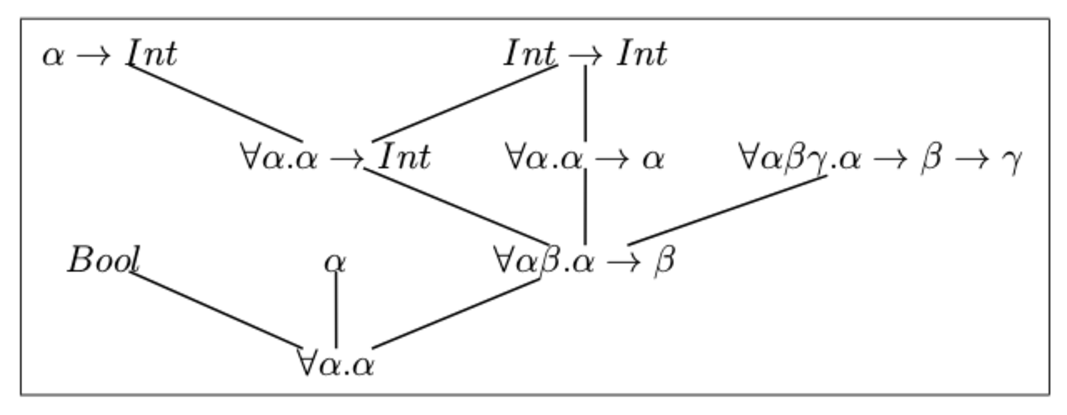
\includegraphics[width=9cm]{type-lattice.pdf}
    \caption{This is the caption.}
    \label{fig:boat1}
\end{figure}
\end{frame}

%%%%%%%%%%%%%%%%%%%%%%%%%%%%%%%%%%%%%%%%%%%%%%%%%%%%%%%%%%

\begin{frame}[fragile]{Type Rules}
\begin{itemize}
    \item A {\it substitution} is a list of pairs denoted as $S = \{\alpha_{1}/\tau_{1} \dots \alpha_{n}/\tau_{n}\}$.
    \item A substitution S applied on a type expression $\sigma$, denoted by S ($\sigma$)\\
involves simultaneous substitution of the variables $\alpha_1\dots\alpha _n$, if\\
they occur free in $\sigma$, by the corresponding type expressions $\tau_1$ 
$\dots\tau_n$.
\begin{definition}Let $\sigma = \forall\alpha_1\dots\alpha_m$.$\tau$ and $\sigma' = \forall\beta_1\dots\beta_n$.$\tau'$. Then $\sigma'$ is a generic
instance of $\sigma$, iff there is a substitution S acting only on $\{\alpha_1\dots\alpha_m\}$
such that $\tau' = S (\tau)$ and no $\beta_i$ is free in $\sigma$.\end{definition}
    \item Clearly, the restriction that no $\beta_i$ is free in $\sigma$ is needed, else we
would have absurdities like $\alpha\to Int\leq\forall\alpha.\alpha\to Int$. 
\end{itemize}
\end{frame}

%%%%%%%%%%%%%%%%%%%%%%%%%%%%%%%%%%%%%%%%%%%%%%%%%%%%%%%%%%

\begin{frame}[fragile]{\textbf{Recapitulation – Type rules for $\lambda_{2}$}}
\begin{equation}
\tag{\textsc{Var}}
\Gamma \cup \{x :: \sigma\} \vdash x :: \sigma
\label{eqn:Var}
\end{equation}

\begin{equation}
\tag{\textsc{Con}}
\Gamma \cup \{c :: \sigma\} \vdash c :: \sigma
\label{eqn:Con}
\end{equation}

\begin{equation}
\tag{\textsc{Inst}}
\frac{\Gamma \vdash M :: \sigma \qquad \sigma^{'} \geq \sigma}{\Gamma \vdash M :: \sigma^{'}}
\label{eqn:Inst}
\end{equation}

\begin{equation}
\tag{\textsc{Gen}}
\frac{\Gamma \vdash M :: \sigma \qquad \alpha \notin FV(\Gamma)}{\Gamma \vdash M :: \forall\alpha.\sigma}
\label{eqn:Gen}
\end{equation}

\begin{equation}
\tag{\textsc{M-App}}
\frac{\Gamma \vdash M :: \tau_{1} \rightarrow \tau_{2}\qquad\Gamma \vdash N :: \tau_{1}}{\Gamma \vdash M\ N :: \tau_{2}}
\label{eqn:M-App}
\end{equation}

\begin{equation}
\tag{\textsc{M-Abs}}
\frac{\Gamma,x :: \tau_{1} \vdash M :: \tau_{2}}{\Gamma \vdash \lambda x.M :: \tau_{1} \rightarrow \tau_{2}}
\label{eqn:M-Abs}
\end{equation}
\end{frame}

%%%%%%%%%%%%%%%%%%%%%%%%%%%%%%%%%%%%%%%%%%%%%%%%%%%%%%%%%%

\begin{frame}[fragile]{\textbf{Hindley-Milner - Type checking variables}}
\setbeamertemplate{enumerate items}[default]
\begin{enumerate}[1:]
\item $t \textbf{ is a variable } x$
\begin{figure}[h]
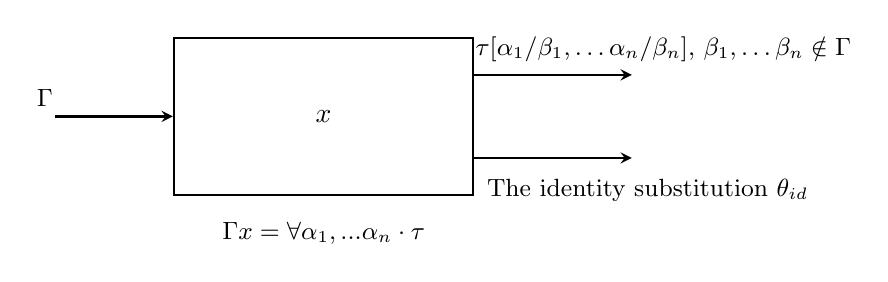
\begin{tikzpicture}[auto,>=latex']
\node[w] (x) {$x$};
\node[font=\fontsize{9}{0}\selectfont, below = 6pt of x] {$\Gamma x = \forall\alpha_{1},...\alpha_{n}\cdot\tau$};
\draw[<-, thick, >=stealth, near end] (x.west) -- node[font=\fontsize{9}{0}\selectfont, above, xshift=-5mm] {$\Gamma$} +(-15mm,0pt);

\draw[->, thick, >=stealth, near end] ([yshift=15pt]x.east) -- node[font=\fontsize{9}{0}\selectfont, above, xshift=9mm, yshift=1pt] {$\tau[\alpha_{1}/\beta_{1},\ldots\alpha_{n}/\beta_{n}],$ $\beta_{1},\ldots\beta_{n}\notin\Gamma$} +(20mm,0pt);

\draw[->, thick, >=stealth] ([yshift=-15pt]x.east) -- node[font=\fontsize{9}{0}\selectfont, below, xshift=12mm, yshift=-4pt] {The identity substitution $\theta_{id}$} +(20mm,0pt);

\end{tikzpicture}
\end{figure}
\begin{itemize}
  \item $\beta_{1},\ldots,\beta_{n}$ are fresh variables.
  \item Reason for monomorphising the type of x: We try to find the type of
  a variable only in the context of an application, and our application
  is monomorphic.
\end{itemize}
\end{enumerate}
\end{frame}

%%%%%%%%%%%%%%%%%%%%%%%%%%%%%%%%%%%%%%%%%%%%%%%%%%%%%%%%%%

\begin{frame}[fragile]{\textbf{Hindley-Milner - Type checking applications}}
\setbeamertemplate{enumerate items}[default]
\begin{enumerate}[1]
    \item Typecheck $e_1$ with the initial environment $\Gamma$. Result is $\tau_1$ and $\theta_1$.
    \item Typecheck $e_2$ with the environment $\theta_1$ $\Gamma$. Result is $\tau_2$ and $\theta_2$.
    \item Unify $\theta_2$ $\tau_1$ and $\tau_2 \to \alpha$. Assume that unifier is $\theta$. And the unified
term ($\theta$ $\alpha$) is $\tau_3$ .
    \item Type of the application is $\tau_3$ and the final substitution is $\theta\circ\theta_2\circ\theta_1$.
\end{enumerate}
\end{frame}

\end{document}
